\section{SiPM radiation damage\label{sec:sipm-rad}}

For the duration of the CRF experiment, the readout modules (RMs) were situated in a rack at z = 14.6 m from the interaction point (IP). Unfortunately, the RMs were not sufficiently protected in this area by the HCAL forward calorimeter radiation shielding, and thus they were exposed to a neutron fluence of the order of 1-2 $\cdot$ 10$^{10}$ per 10 fb$^{-1}$ as calculated by FLUKA simulations. As a result, the single-photoelectron peak spectra of the SiPMs degraded progressively after the first day of the CRF study, becoming noisier and less distinct with increasing exposure to the ambient radiation.

The CRF RMs were installed on the rack on September 14, 2016. From pedestal runs taken on that day, clear and distinct dark-current and single-photoelectron peaks could be observed in the pulse size spectra of all channels (see Figure~\ref{fig:spe-peaks} top left), and the gain distribution for all the SiPMs had a mean of 47.44 fC with a spread of 2\% (Fig~\ref{fig:gaindistr}).

\begin{figure}[hbtp]
\begin{center}
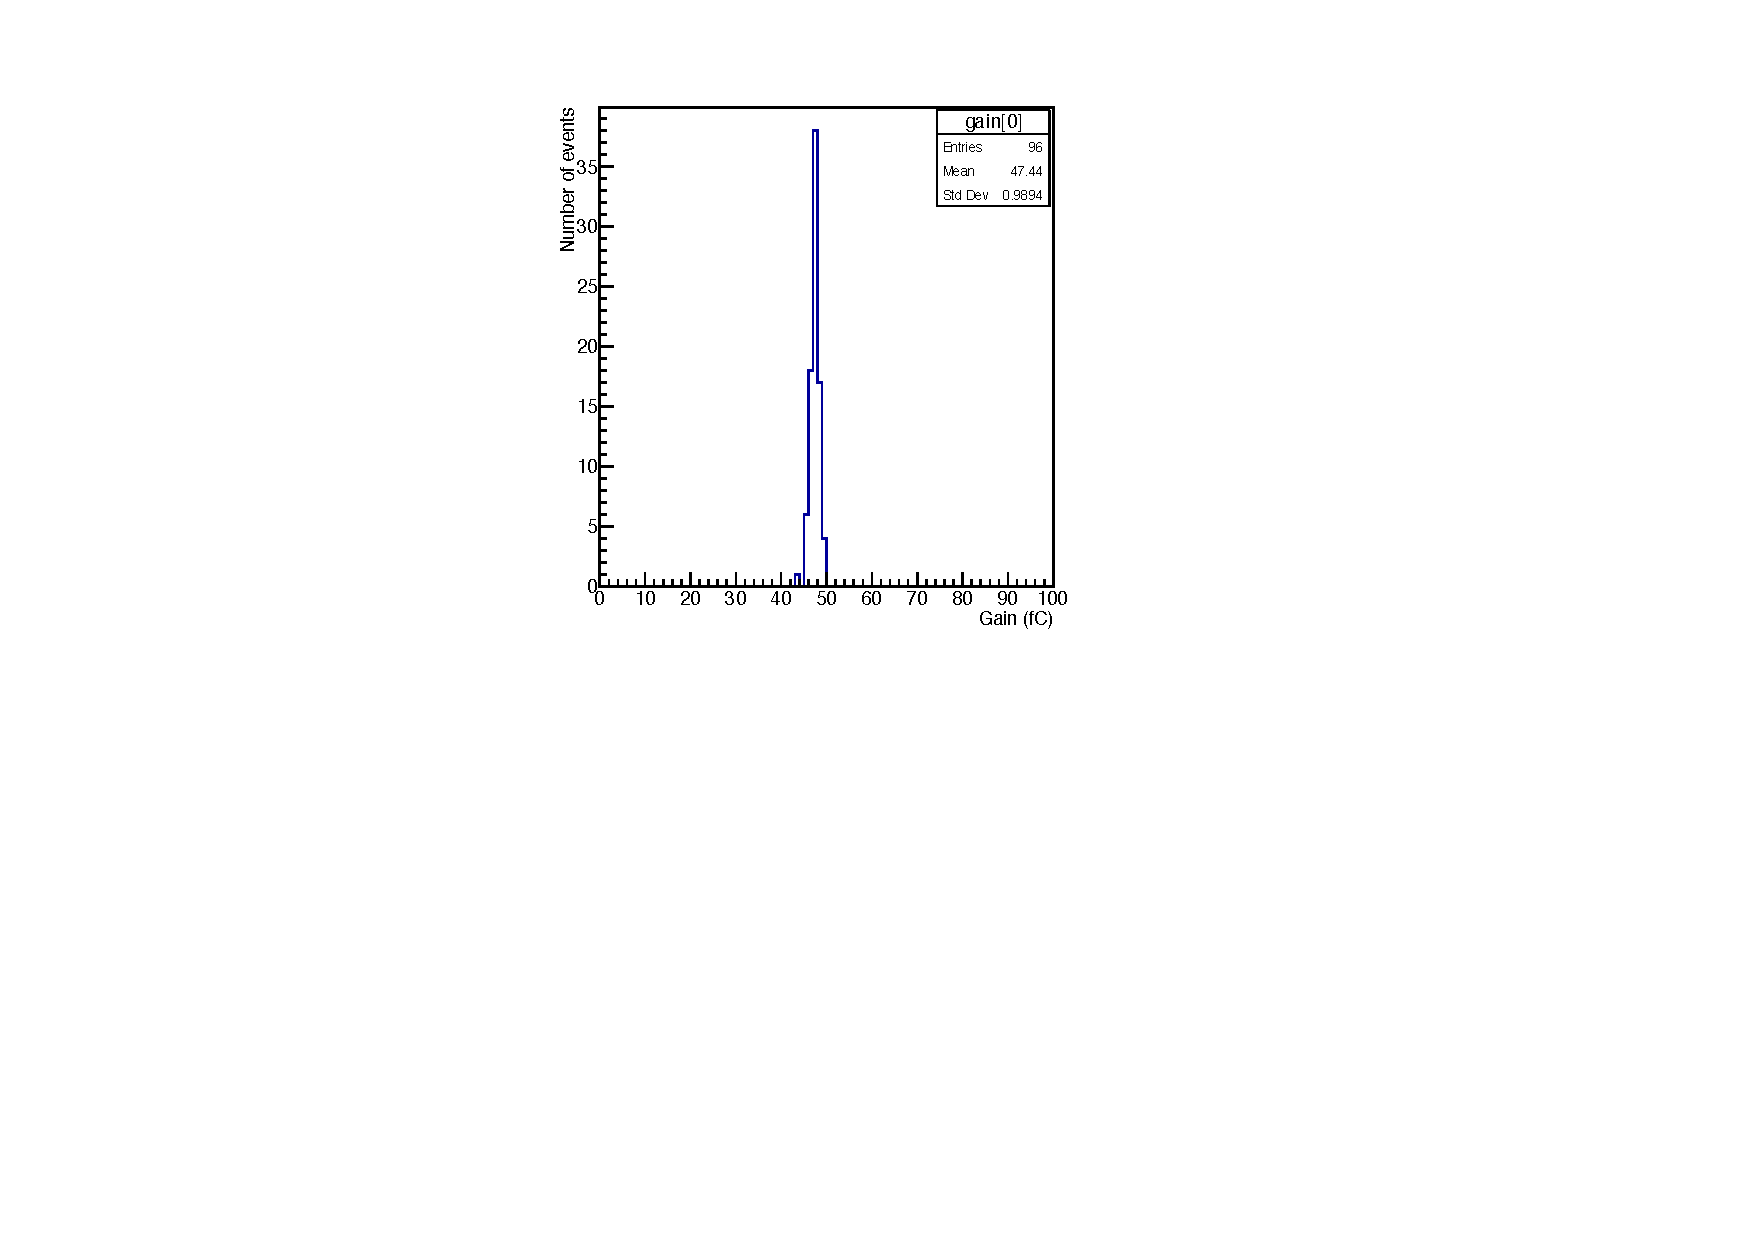
\includegraphics[width=0.75\textwidth]{figures/Run280646_RM1and2_Gains}
\caption{Gain distribution for all SiPMs (total of 96) in the two CRF readout modules (RM). Gains were calculated by fitting Gaussian peaks to the pulse size spectra of each RM channel in a pedestal run and subtracting the fitted pedestal mean.}
\label{fig:gaindistr}
\end{center}
\end{figure}

Another pedestal run was taken on September 28, 2016, after 1.1 fb$^{-1}$ of integrated luminosity since the CRF system was set up. The pulse size spectra for this run (see Figure~\ref{fig:spe-peaks} top right) show considerably more noise compared to the pedestal run taken on the first day; in this run, the single-photoelectron peaks are larger with respect to the dark-current peak, indicating more noise in the SiPMs.

A pedestal run taken on October 1, 2016, at 2.1 fb$^{-1}$ of integrated luminosity, shows (see Figure~\ref{fig:spe-peaks} bottom left) that the dark-current and single-photoelectron peaks have blurred into one another and become indistinct.

This trend continued throughout the irradiation of the CRF system during the proton-proton runs in the following months. A pedestal run from October 28, 2016, at the end of proton-proton data-taking for the year, shows (see Figure~\ref{fig:spe-peaks} bottom right) that the single-photolectron peaks in the pulse size spectrum are still impossible to discern, and that the average amount of noise in the SiPMs is of the order of 1000 fC integrated over a window of 4 consecutive time-slices.

The following plot (\textbf{PLOT NEEDED!}) shows the average dark current or SiPM noise for a few randomly-selected empty channels as a function of time. The SiPM noise grows steadily until the end of proton-proton data-taking in October 28, after which the SiPM noise is seen to decrease steadily.

\begin{figure}[hbtp]
\begin{center}
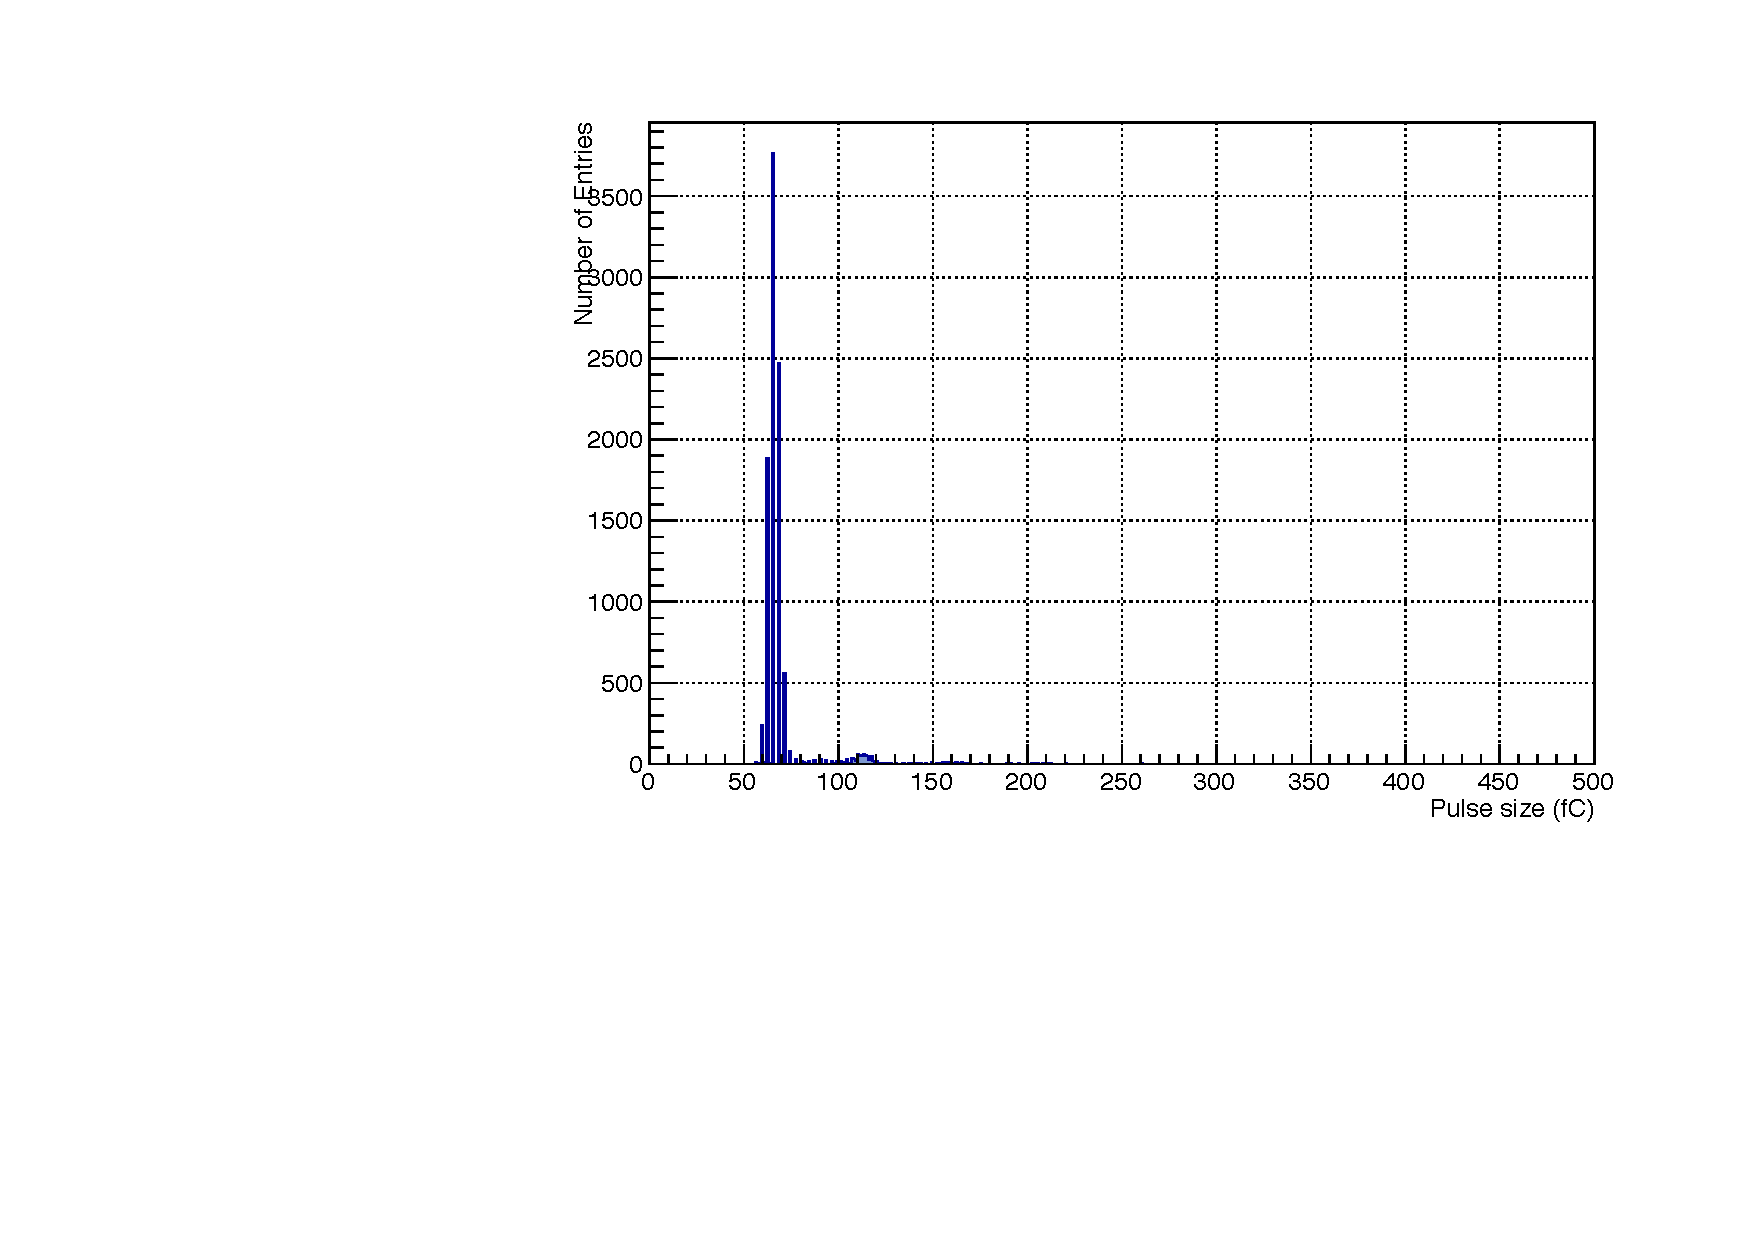
\includegraphics[width=0.4\textwidth]{figures/PulseSizeSpectrum_0fb}
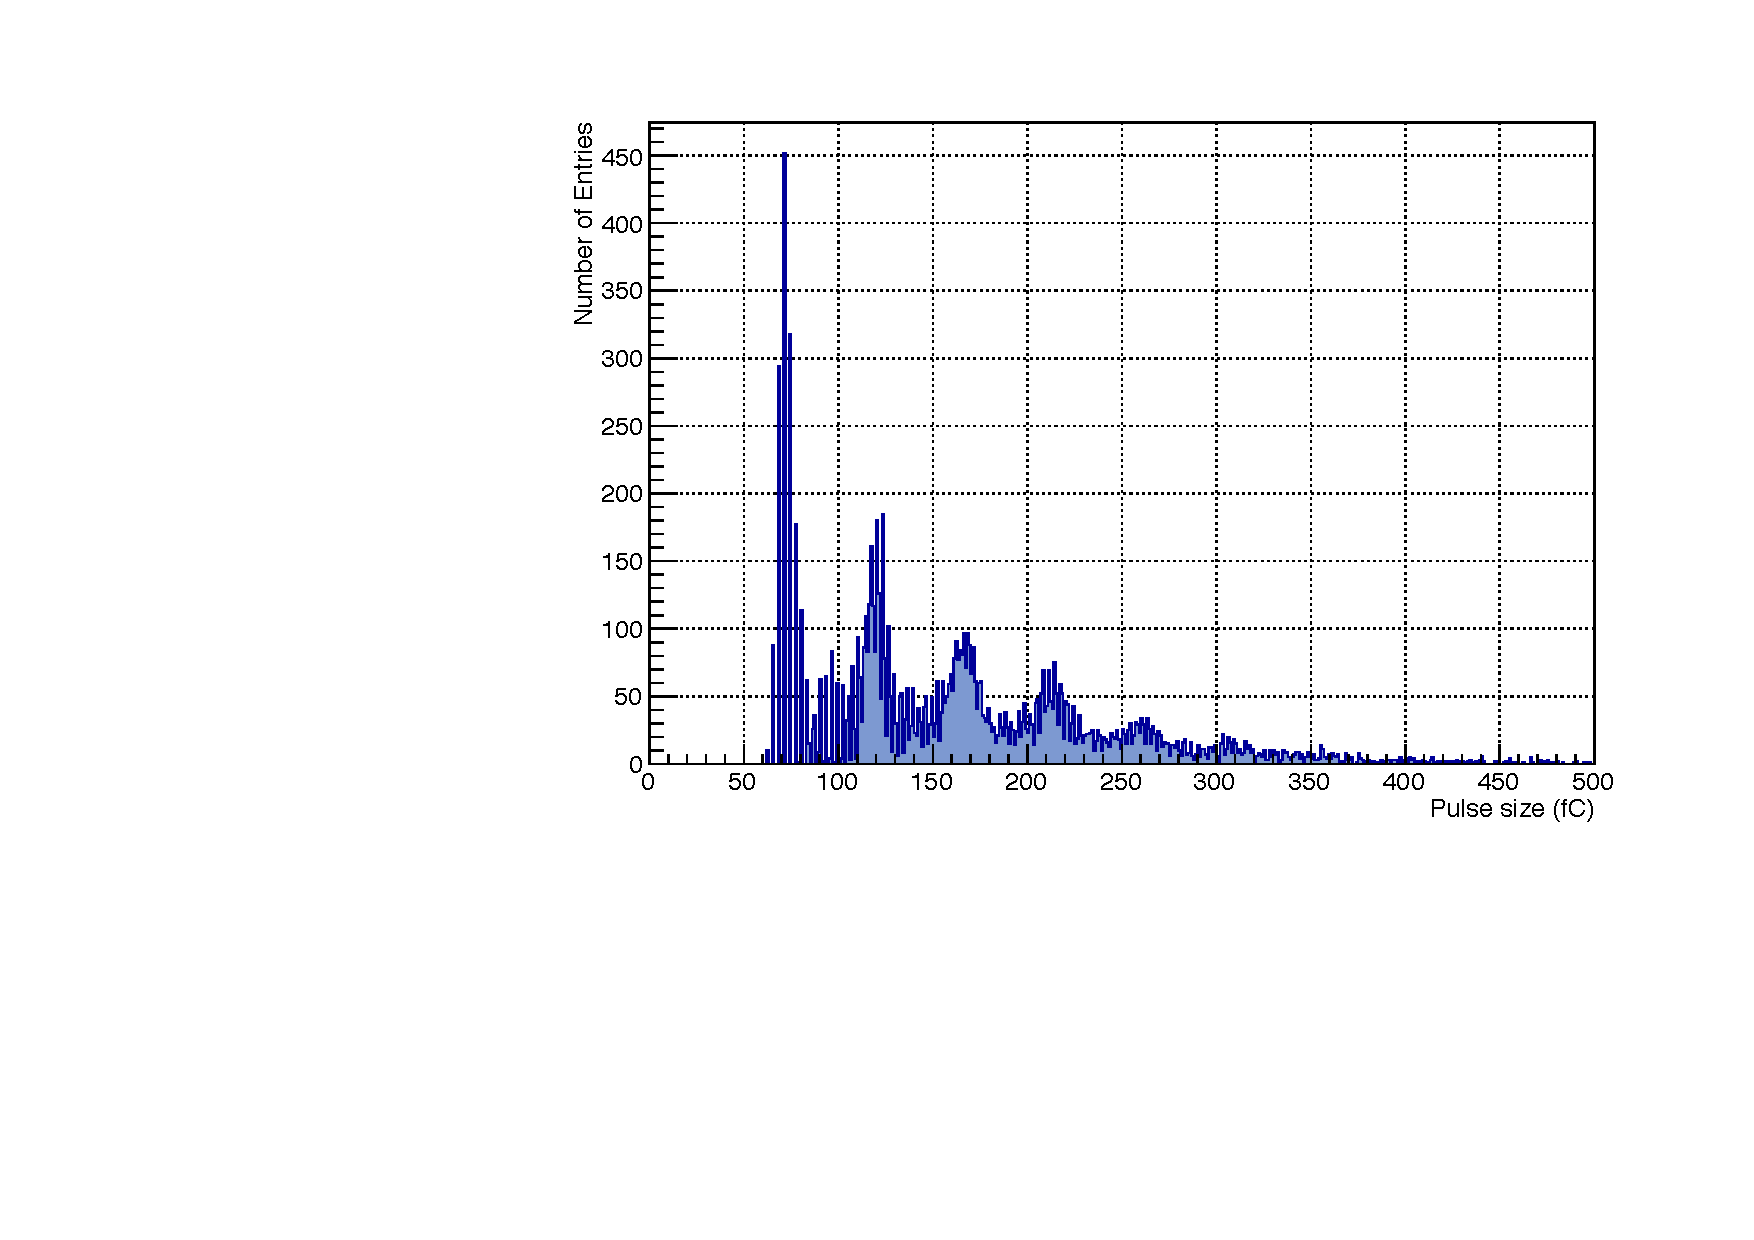
\includegraphics[width=0.4\textwidth]{figures/PulseSizeSpectrum_1fb}
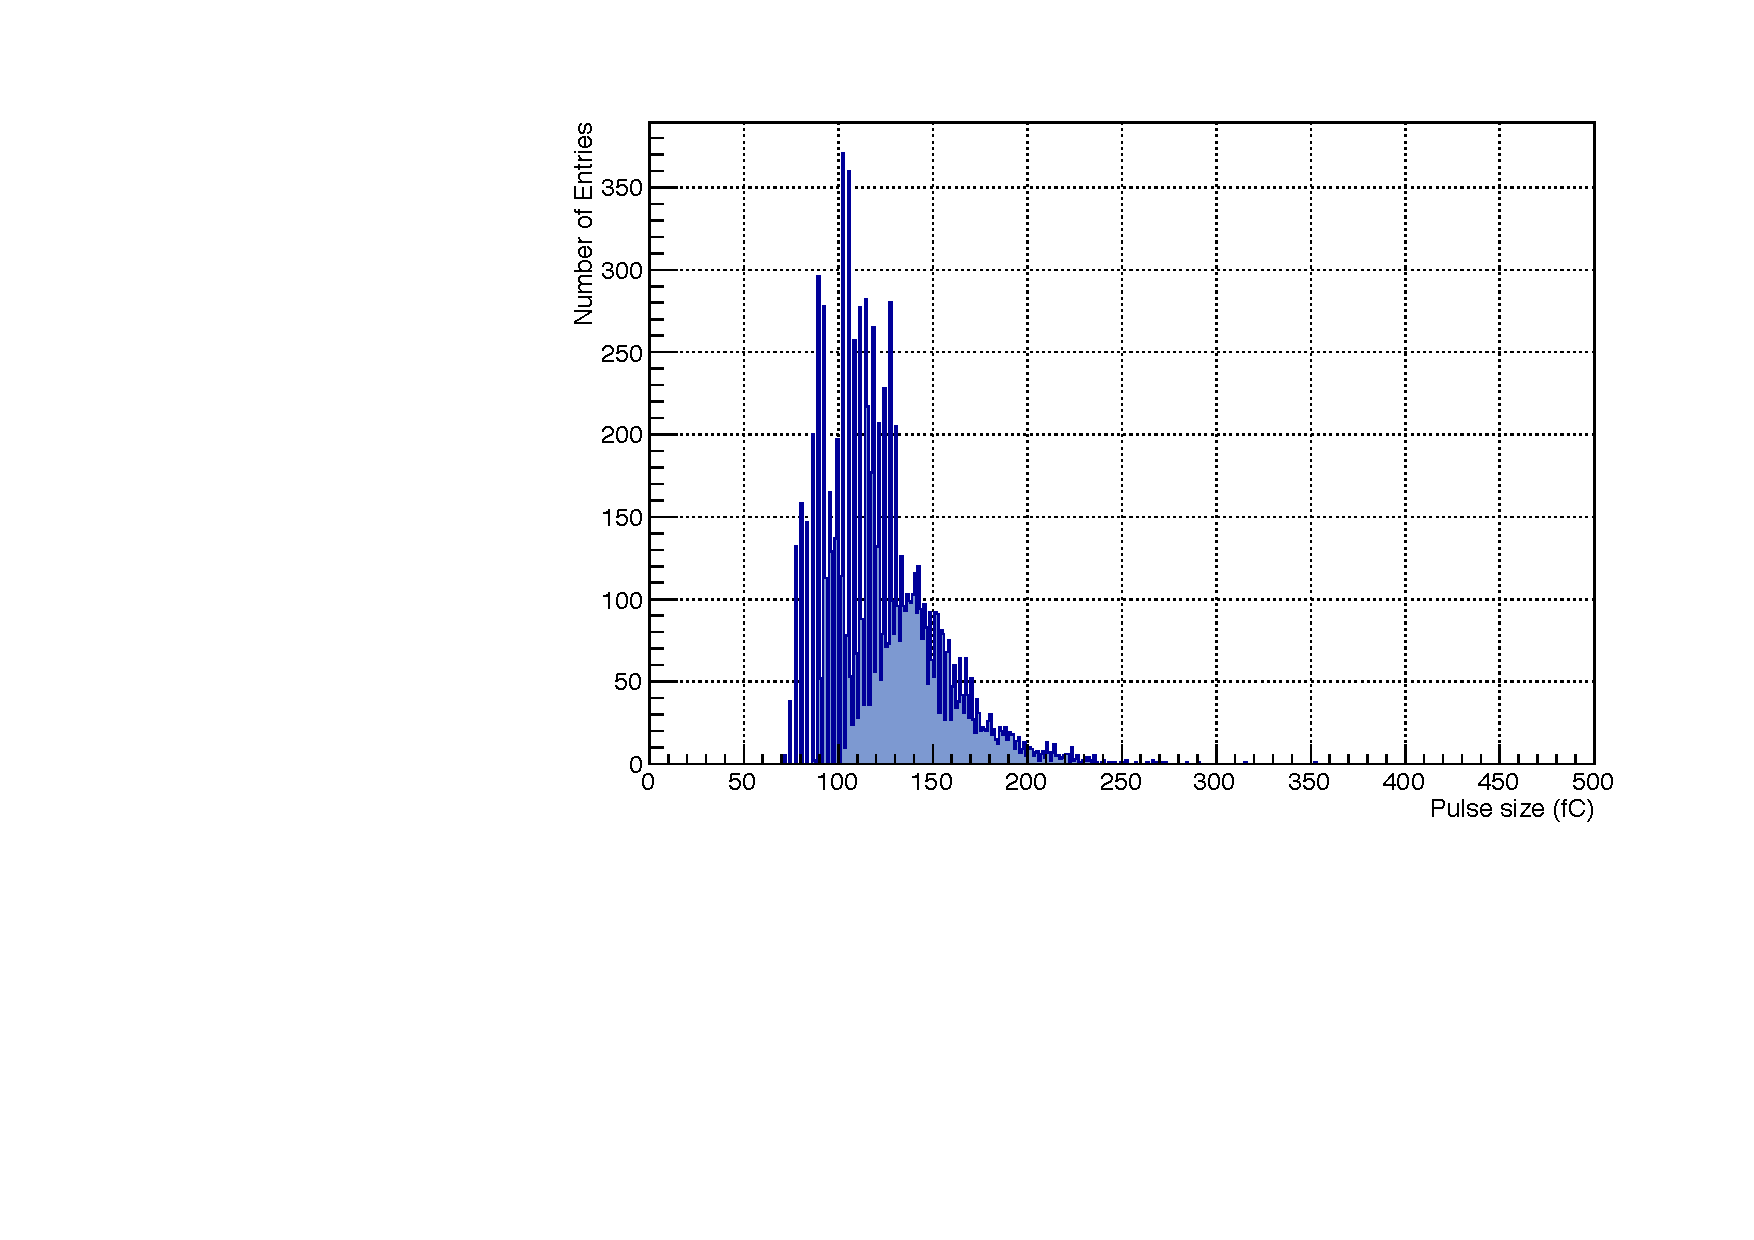
\includegraphics[width=0.4\textwidth]{figures/PulseSizeSpectrum_2fb}
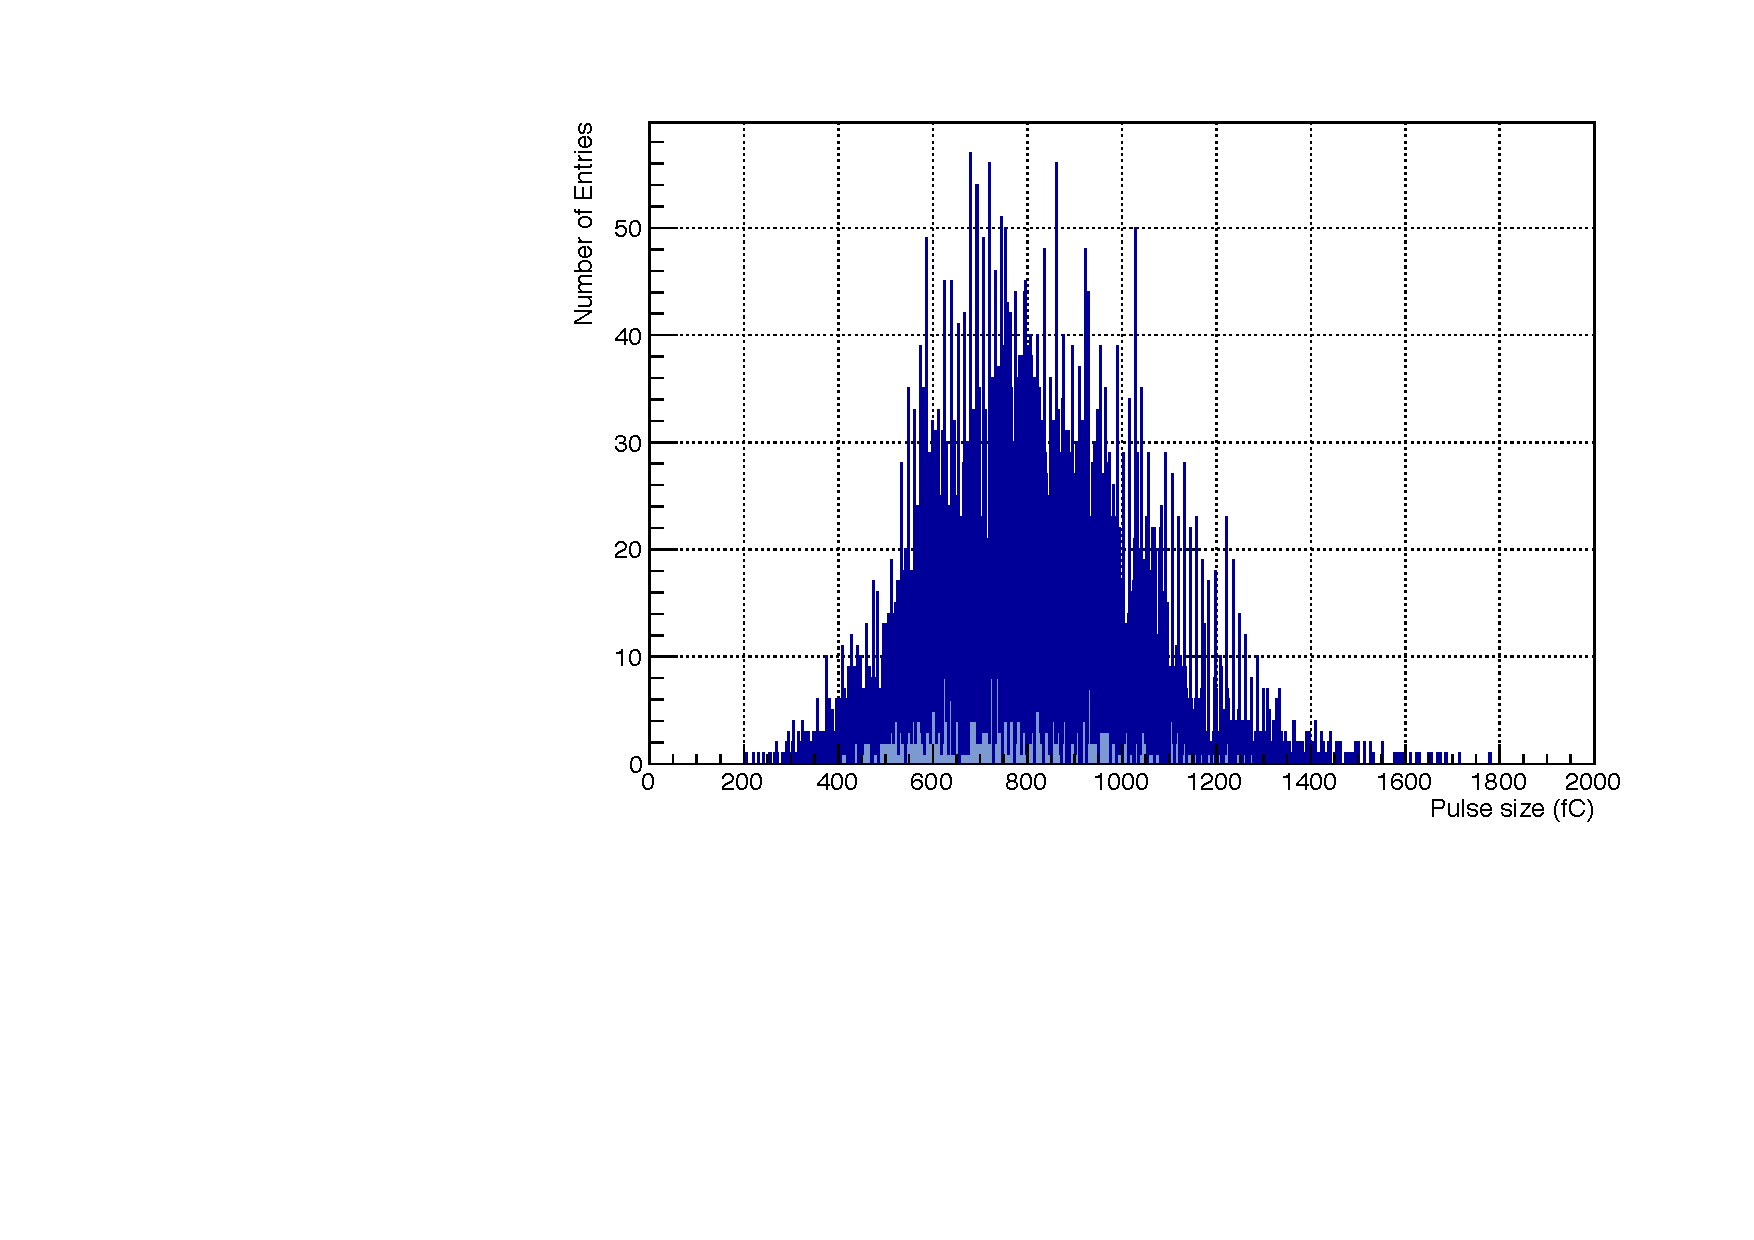
\includegraphics[width=0.4\textwidth]{figures/PulseSizeSpectrum_10fb}
\caption{(Top left) Pulse size spectrum before any irradiation (0 fb$^{-1}$), in one representative channel from the CRF RMs. (Top right) Pulse size spectrum after 1.1 fb$^{-1}$. (Bottom left) Pulse size spectrum after 2.1 fb$^{-1}$. (Bottom right) Pulse size spectrum after 10 fb$^{-1}$.}
\label{fig:spe-peaks}
\end{center}
\end{figure}


Observations:
\begin{itemize}
\item Because of the blurring of the single-photoelectron peaks due to radiation damage to the SiPMs, the SiPM gains cannot be calculated for any pedestal runs aside from the ones taken on September 28 and October 1. This loss of information about the SiPM gains in any of the subsequent runs introduces a systematic uncertainty in the size of the signals measured; an estimate of this uncertainty is needed.
\item The fact that the SiPM noise began to decrease after the end of the irradiation period suggests that there was some recovery process occurring in the SiPMs.


For a future iteration of this radiation damage study, the RMs must be placed in an area with at least 10 times less neutron flux, in order to avoid damaging the SiPMs.

\end{itemize}
